% Figure 2.1 (Session 2): the two ends of the XXZ chain, the Neel pair and the singlet coverings.
% The image is rendered by figures/blender/s2_1_neel_pair.py; the coordinates of the labels
% come from figures/blender/out/neel_pair_anchors.tex. Compile with:
%   pdflatex neel_pair.tex ; result moves to ../quantum_magnetism/neel_pair.pdf
\documentclass[11pt,tikz,border=0pt]{standalone}
\usepackage{amsmath,amssymb,graphicx,braket}
\usepackage{xcolor}
\definecolor{coursedark}{HTML}{1B2A4A}
\definecolor{costamber}{HTML}{B8620A}
\newlength{\figw}\setlength{\figw}{16.19cm}   % the text width of the notes (letter, 2.7 cm margins), so labels print at size
\newcommand{\up}{\uparrow}\newcommand{\dn}{\downarrow}

\begin{document}
\begin{tikzpicture}[lbl/.style={font=\small, text=coursedark}]
  \node[anchor=south west, inner sep=0pt] at (0,0)
    {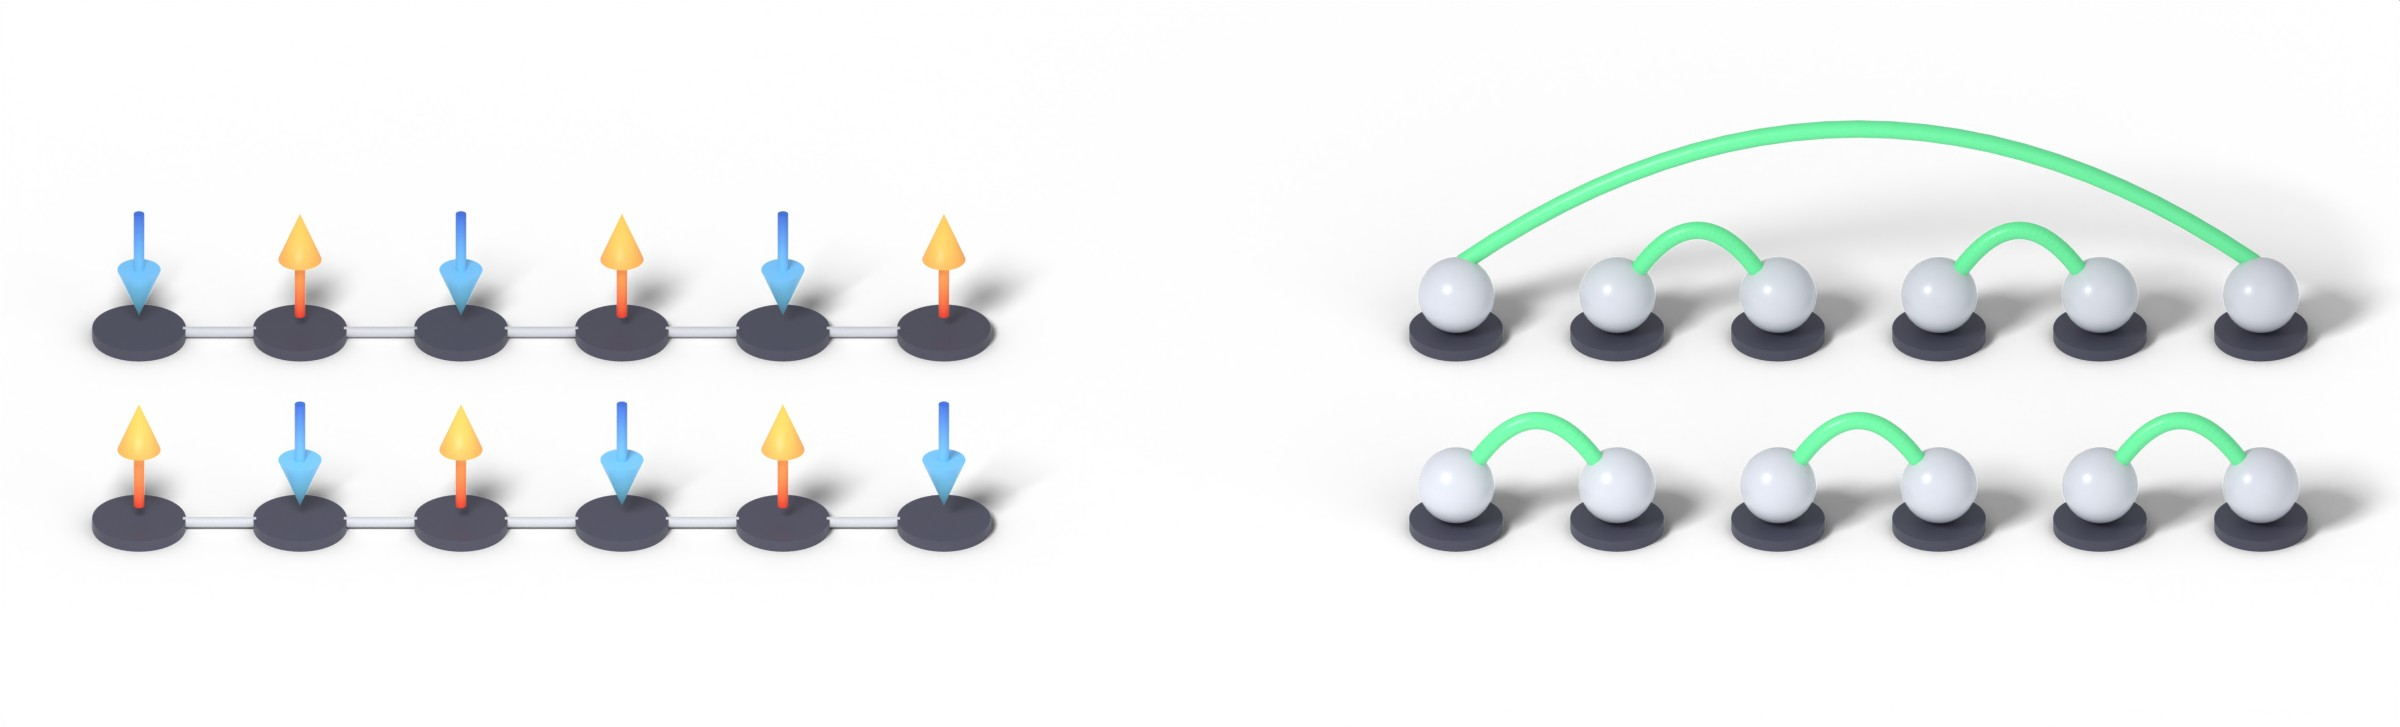
\includegraphics[width=\figw]{../blender/out/neel_pair.jpg}};
  %% written by figlib.py; x and y in units of the image width
\coordinate (a) at (0.0274\figw,0.2545\figw);
\coordinate (ketA) at (0.4177\figw,0.1092\figw);
\coordinate (ketB) at (0.4177\figw,0.1885\figw);
\coordinate (b) at (0.5762\figw,0.2545\figw);
\coordinate (plus) at (0.5823\figw,0.1409\figw);
\coordinate (chainA) at (0.2256\figw,0.0553\figw);
\coordinate (chainB) at (0.7744\figw,0.0553\figw);

  \node[lbl, font=\normalsize, anchor=west] at (a) {(a)};
  \node[lbl, font=\normalsize, anchor=west] at (b) {(b)};
  \node[lbl, anchor=west] at (ketA) {$\ket{\up\dn\up\dn\cdots}$};
  \node[lbl, anchor=west] at (ketB) {$\ket{\dn\up\dn\up\cdots}$};
  \node[lbl, font=\normalsize] at (plus) {$+$};
  \node[lbl, anchor=north] at (chainA) {Ising end, $J_{xy}=0$};
  \node[lbl, anchor=north] at (chainB) {Heisenberg end, $J_{xy}=J_z$};
\end{tikzpicture}
\end{document}
